% Included from both -slides and -handout versions.

\mode<presentation>
{
  \usetheme{default}
  \useoutertheme{infolines}
}

\usepackage[english]{babel}
\usepackage[latin1]{inputenc}
\usepackage{graphicx}
\usepackage{times}
\usepackage[T1]{fontenc}
\usepackage{fancyvrb}
\usepackage{hyperref}
\usepackage{listings}
\begin{document}
\lstset{language=C, escapeinside={(*@}{@*)}, numbers=left,
  basicstyle=\tiny, showspaces=false, showtabs=false}

\title{L41: Kernels and Tracing}
%\subtitle{Through tracing, analysis, and experimentation}
%\institute{University of Cambridge}
%\author{George V. Neville-Neil}
\author{Dr Robert N. M. Watson}
\date{15 October 2015}

\begin{frame}
  \titlepage
\end{frame}

\section{Introduction}

\begin{frame}
  \frametitle{Reminder: last time}

  \begin{enumerate}
    \item What is an operating system?
    \item Systems research
    \item About the module
    \item Lab reports
  \end{enumerate}
\end{frame}

\begin{frame}
  \frametitle{This time: Tracing the kernel}

  \begin{enumerate}
    \item DTrace
    \item The probe effect
    \item The kernel: Just a C program?
    \item A little on kernel dynamics: How work happens
  \end{enumerate}
\end{frame}

\section{DTrace}

\begin{frame}
  \frametitle{Dynamic tracing with DTrace}

  \begin{itemize}
    \item Bryan M. Cantrill, Michael W. Shapiro, and Adam H. Leventhal.
      \textit{Dynamic Instrumentation of Production Systems},
      USENIX Annual Technical Conference, USENIX, 2004.

    \pause

    \begin{itemize}
      \item ``Facility for dynamic instrumentation of production systems''
      \item Unified and safe instrumentation of kernel and userspace
      \item Zero \textit{probe effect} when not enabled

      \pause

      \item Dozens of `providers' representing different trace sources
      \item Tens (hundreds?) of thousands of instrumentation points

      \pause

      \item C-like high-level control language with predicates and actions
      \item User-defined variables, thread-local variables, associative arrays
      \item Data aggregation and speculative tracing
    \end{itemize}

    \pause

    \item Adopted in Solaris, Mac OS X, and FreeBSD; module for Linux
    \item Heavy influence on Linux SystemTap
    \item \textbf{Our tool of choice for this module}
  \end{itemize}
\end{frame}

\begin{frame}[fragile]
  \frametitle{DTrace scripts}

  \begin{itemize}
    \item Human-facing C-like language
    \item One or more \{\textit{probe name}, \textit{predicate},
      \textit{action}\} tuples
    \item Expression limited to control side effects (e.g., no loops)
    \item Specified on command line or via a \texttt{.d} file
  \end{itemize}

  \pause
  \smallskip

  \begin{small}
\begin{verbatim}
fbt::malloc:entry /execname == "csh"/ { trace(arg0); }
\end{verbatim}
  \end{small}

  \smallskip

  \begin{description}
    \item[probe name] Identifies the probe(s) to instrument; wildcards
      allowed; identifies the \textit{provider} and a provider-specific
      \textit{probe name}
    \item[predicate] Filters cases where action will execute
    \item[action] Describes tracing operations
  \end{description}

\end{frame}

\begin{frame}[fragile]
  \frametitle{D Intermediate Format (DIF)}

  \begin{small}
\begin{verbatim}
root@beaglebone:/data # dtrace -Sn
  'fbt::malloc:entry /execname == "csh"/ { trace(arg0); }'
\end{verbatim}
  \end{small}

  \pause

  \begin{tiny}
\begin{verbatim}
DIFO 0x0x8047d2320 returns D type (integer) (size 4)
OFF OPCODE      INSTRUCTION
00: 29011801    ldgs DT_VAR(280), %r1		! DT_VAR(280) = "execname"
01: 26000102    sets DT_STRING[1], %r2		! "csh"
02: 27010200    scmp %r1, %r2
03: 12000006    be   6
04: 0e000001    mov  %r0, %r1
05: 11000007    ba   7
06: 25000001    setx DT_INTEGER[0], %r1		! 0x1
07: 23000001    ret  %r1

NAME             ID   KND SCP FLAG TYPE
execname         118  scl glb r    string (unknown) by ref (size 256)
\end{verbatim}
  \end{tiny}

\pause

  \begin{tiny}
\begin{verbatim}
DIFO 0x0x8047d2390 returns D type (integer) (size 8)
OFF OPCODE      INSTRUCTION
00: 29010601    ldgs DT_VAR(262), %r1		! DT_VAR(262) = "arg0"
01: 23000001    ret  %r1

NAME             ID   KND SCP FLAG TYPE
arg0             106  scl glb r    D type (integer) (size 8)
\end{verbatim}
  \end{tiny}
\end{frame}

\begin{frame}
  \frametitle{Some kernel DTrace providers in FreeBSD}

  \begin{center}
  \begin{small}
  \begin{tabular}{ll}
    \hline
      \textbf{Provider} & \textbf{Description} \\
    \hline
      \texttt{callout\_execute} & Timer-driven callouts \\
      \texttt{dtmalloc} & Kernel \texttt{malloc()}/\texttt{free()} \\
      \texttt{dtrace} & DTrace script events (\texttt{BEGIN}, \texttt{END}) \\
      \texttt{fbt} & Function Boundary Tracing \\
      \texttt{io} & Block I/O \\
      \texttt{ip}, \texttt{udp}, \texttt{tcp}, \texttt{sctp}  & TCP/IP \\
      \texttt{lockstat} & Locking \\
      \texttt{proc}, \texttt{sched} & Kernel process/scheduling \\
      \texttt{profile} & Profiling timers \\
      \texttt{syscall} & System call entry/return \\
      \texttt{vfs} & Virtual filesystem \\
    \hline
  \end{tabular}
  \end{small}
  \end{center}

  \begin{itemize}
    \item Providers represent data sources -- types of instrumentation
    \item Apparent duplication: FBT vs. event-class providers?
    \begin{itemize}
      \item Efficiency, expressivity, interface stability, portability
    \end{itemize}
  \end{itemize}

\end{frame}

\begin{frame}[fragile]
  \frametitle{Tracing kernel \texttt{malloc()} calls}

  \begin{itemize}
    \item Trace first argument to kernel \texttt{malloc()} for \texttt{csh}
    \item Note: captures both successful and failed allocations
  \end{itemize}

  \begin{small}
\begin{verbatim}
root@beaglebone:/data # dtrace -n
  'fbt::malloc:entry /execname=="csh"/ { trace(arg0); }'
\end{verbatim}
  \end{small}

  \begin{description}
    \item[Probe] Use FBT to instrument \texttt{malloc()} prologue
    \item[Predicate] Limit actions to processes executing \texttt{csh}
    \item[Action] Trace the first argument (\texttt{arg0})
  \end{description}

  \pause

  \begin{small}
\begin{verbatim}
CPU     ID          FUNCTION:NAME
  0   8408           malloc:entry        64
  0   8408           malloc:entry      2748
  0   8408           malloc:entry        48
  0   8408           malloc:entry       392
^C
\end{verbatim}
  \end{small}
\end{frame}

\begin{frame}
  \frametitle{Aggregations}

  \begin{itemize}
    \item Often we want summaries of events, not detailed traces
    \item DTrace allows early, efficient \textit{reduction} using aggregations
  \end{itemize}

  \pause

  \begin{center}
    \begin{small}
      \begin{tabular}{ll}
        \hline
        Aggregation & Description \\
        \hline
	\texttt{count()} & Number of times called \\
	\texttt{sum()} & Sum of arguments \\
	\texttt{avg()} & Average of arguments \\
	\texttt{min()} & Minimum of arguments \\
	\texttt{max()} & Maximum of arguments \\
	\texttt{stddev()} & Standard deviation ofnts \\
	\texttt{lquantize()} & Linear frequency distribution (histogram) \\
	\texttt{quantize()} & Log frequency distribution (histogram) \\
        \hline
      \end{tabular}
    \end{small}
  \end{center}

  \pause

  \begin{itemize}
    \item Scalable multicore implementations (i.e., commutative)
    \item \texttt{@variable = function()}; \texttt{printa()} to print
  \end{itemize}

\end{frame}

\begin{frame}[fragile]
  \frametitle{Profiling kernel \texttt{malloc()} calls by \texttt{csh}}

  \begin{small}
\begin{verbatim}
root@beaglebone:/data # dtrace -n 'fbt::malloc:entry
  /execname=="csh"/ { @traces[stack()] = count(); }'
\end{verbatim}
  \end{small}

  \begin{description}
    \item[Probe] Use FBT to instrument \texttt{malloc()} prologue
    \item[Predicate] Limit actions to processes executing \texttt{csh}
    \item[Action] Keys of associative array are stack traces
      (\texttt{stack()}); \\
      values are aggregated counters (\texttt{count()})
  \end{description}

  \pause

  \begin{small}
\begin{verbatim}
^C
              kernel`malloc
              kernel`fork1+0x14b4
              kernel`sys_vfork+0x2c
              kernel`swi_handler+0x6a8
              kernel`swi_exit
              kernel`swi_exit
                3
...
\end{verbatim}
\end{small}
\end{frame}

\begin{frame}
  \frametitle{DTrace: implementation}

  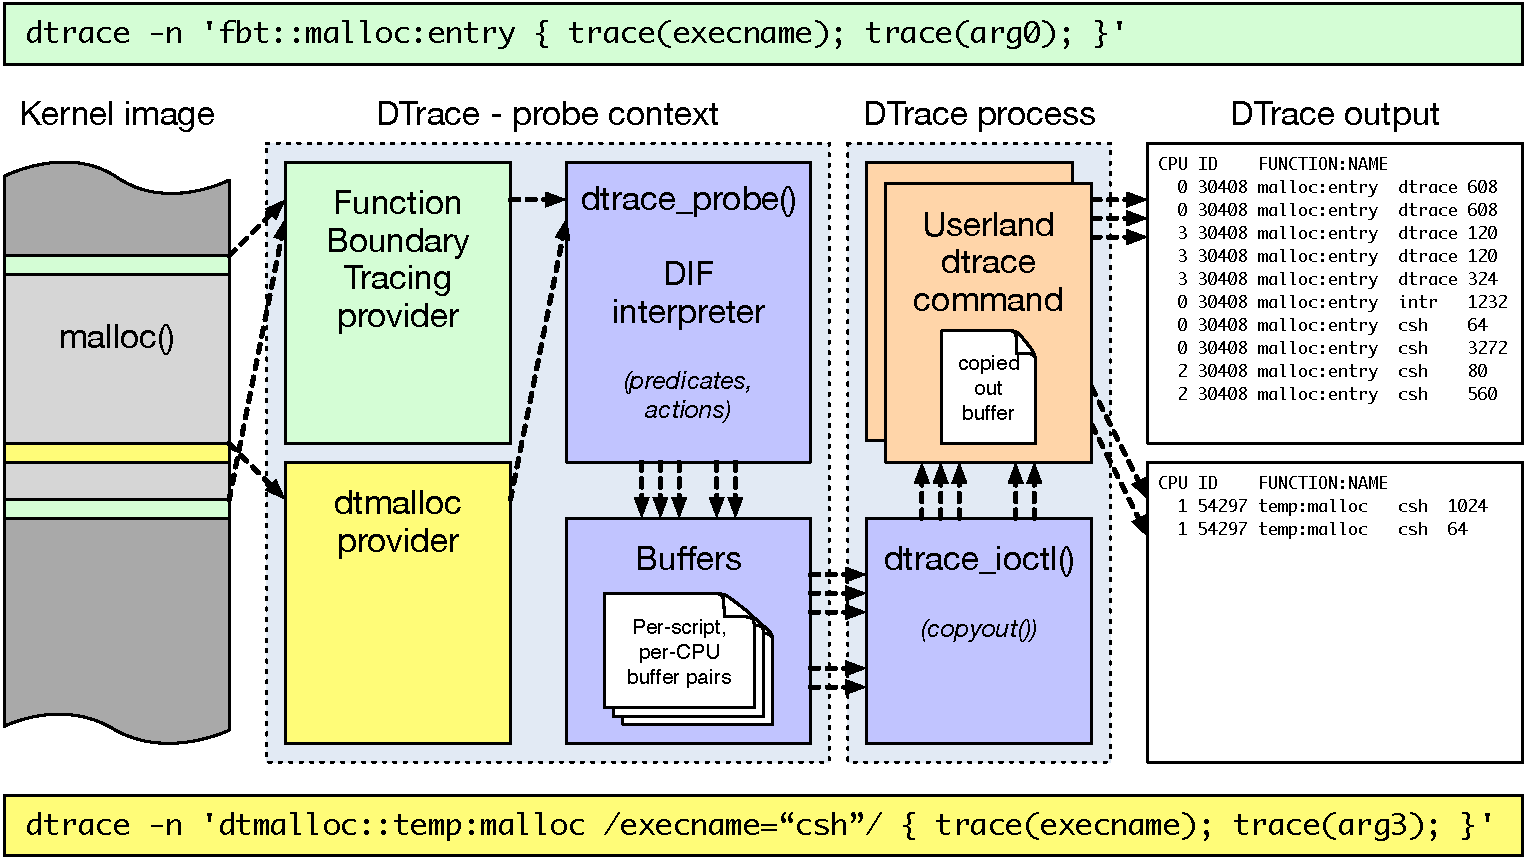
\includegraphics[width=\textwidth]{../../figures/dtrace-the-big-picture.pdf}
\end{frame}

\begin{frame}
  \frametitle{The `probe effect'}

  \begin{itemize}
    \item The \textit{probe effect} is the unintended alteration in system
      behaviour that arises from measurement
    \item Why?  Software instrumentation is \textit{active}: execution is
      changed

    \pause
    \medskip

    \item DTrace minimises \textit{probe effect} when not being used...
    \begin{itemize}
      \item ... but has a very significant impact when it is
      \item Disproportionate effect on probed events
    \end{itemize}

    \pause
    \medskip

    \item Potential perturbations:
    \begin{itemize}
      \item Execution speed relative to other cores (e.g., lock hold times)
      \item Execution speed relative to external events (e.g., timer ticks)
      \item Microarchitectural effects (e.g., cache footprint, branch predictor)
    \end{itemize}

    \pause
    \medskip

    \item What does this mean for us?
    \begin{itemize}
      \item Don't benchmark while running DTrace ...
      \item ... unless benchmarking DTrace
      \item Be aware that traced application may behave differently
      \item E.g., more timer ticks will fire, I/O will ``seem faster''
    \end{itemize}

  \end{itemize}
\end{frame}

\begin{frame}[fragile]
  \frametitle{Probe effect example: \texttt{dd} execution time}

  \begin{itemize}
    \item Simple (naive) microbenchmark
    \item \texttt{dd(1)} copies blocks from an input to an output
    \item Copy one 10M buffer from \texttt{/dev/zero} to \texttt{/dev/null}
    \item Execution time measured with \texttt{/usr/bin/time}
  \end{itemize}

  \medskip
  \pause

  \begin{small}
\begin{verbatim}
# dd if=/dev/zero of=/dev/null bs=10m count=1 status=none
\end{verbatim}
  \end{small}

    \medskip
    \pause

  \begin{itemize}
    \item Simultaneously, run various DTrace scripts
    \item Compare resulting execution times using \texttt{ministat}
  \end{itemize}
\end{frame}

\begin{frame}[fragile]
  \frametitle{Probe effect example 1: Memory allocation}

  \begin{itemize}
    \item Using the \texttt{dtmalloc} provider, count kernel memory allocations
  \end{itemize}

  \pause

  \begin{small}
\begin{verbatim}
dtmalloc::: { @count = count(); }
\end{verbatim}
  \end{small}

  \pause

  \begin{center}
    \begin{tiny}
      \begin{verbatim}
% ministat no-dtrace dtmalloc-count
x no-dtrace
+ dtmalloc-count
+------------------------------------------------------------------------------+
|                                      *                                       |
|                                      *                                       |
|                                      *                                      +|
|x                                     *                                      +|
|x                                     *                                      +|
|*                                     *                                      *|
|        |_______________|______A______M__________A_____|__________________|   |
+------------------------------------------------------------------------------+
    N           Min           Max        Median           Avg        Stddev
x  11           0.2          0.22          0.21    0.20818182  0.0060302269
+  11           0.2          0.22          0.21    0.21272727  0.0064666979
No difference proven at 95.0% confidence
\end{verbatim}
      \end{tiny}
  \end{center}

  \begin{itemize}
    \item No statistically significant overhead at 95\% confidence level
  \end{itemize}
\end{frame}

\begin{frame}[fragile]
  \frametitle{Probe effect example 2: Locking operations}

  \begin{itemize}
    \item \texttt{lockstat} provider tracks lock acquire, release, ...
    \item 6 calls to \texttt{malloc}, but 170K locking operations!
  \end{itemize}

  \begin{small}
    \begin{verbatim}
lockstat::: { @count = count(); }
\end{verbatim}
  \end{small}

  \pause

  \begin{center}
    \begin{tiny}
\begin{verbatim}
ministat no-dtrace lockstat-count
x no-dtrace
+ lockstat-count
+------------------------------------------------------------------------------+
|   x                                                                         +|
|   x                                                                         +|
|   x                                                                     +   +|
|x  x                                                                     +   +|
|x  x                                                                     +   +|
|x  x  x                                                               +  +   +|
| |_A_|                                                                   |_A_M|
+------------------------------------------------------------------------------+
    N           Min           Max        Median           Avg        Stddev
x  11           0.2          0.22          0.21    0.20818182  0.0060302269
+  11          0.42          0.44          0.44    0.43454545  0.0068755165
Difference at 95.0% confidence
	0.226364 +/- 0.00575196
	108.734% +/- 2.76295%
	(Student's t, pooled s = 0.0064667)
\end{verbatim}
    \end{tiny}
  \end{center}

  \begin{itemize}
    \item 109\% overhead to count all \texttt{lockstat} probes!
  \end{itemize}
\end{frame}

\begin{frame}[fragile]
  \frametitle{Probe effect example 2: Limiting to \texttt{dd}?}

  \begin{itemize}
    \item Limit \texttt{action} to processes with name \texttt{dd}
  \end{itemize}

  \begin{small}
    \begin{verbatim}
lockstat::: /execname == "dd"/ { @count = count(); }
\end{verbatim}
  \end{small}

  \pause

  \begin{center}
    \begin{tiny}
      \begin{verbatim}
ministat no-dtrace lockstat-count-dd 
x no-dtrace
+ lockstat-count-dd
+------------------------------------------------------------------------------+
|                                                                           +  |
|  x                                                                        +  |
|  x                                                                        +  |
|  x                                                                        +  |
|  x                                                                        +  |
|x x                                                                        +  |
|x x                                                                        +  |
|x x x                                                                  + + + +|
||_A|                                                                     |_A| |
+------------------------------------------------------------------------------+
    N           Min           Max        Median           Avg        Stddev
x  11           0.2          0.22          0.21    0.20818182  0.0060302269
+  11          0.54          0.57          0.56    0.55818182  0.0075075719
Difference at 95.0% confidence
	0.35 +/- 0.0060565
	168.122% +/- 2.90924%
	(Student's t, pooled s = 0.00680908)
\end{verbatim}
    \end{tiny}
  \end{center}

  \begin{itemize}
    \item Well, crumbs.  Now the overhead is 168\%!
  \end{itemize}
\end{frame}

\begin{frame}[fragile]
  \frametitle{Probe effect example 3: Locking stack traces}

  \begin{itemize}
    \item Gather more information in \texttt{action}: capture call stacks
  \end{itemize}

  \begin{small}
    \begin{verbatim}
lockstat::: { @stacks[stack()] = count(); }
lockstat::: /execname == "dd"/ { @stacks[stack()] =
  count(); }
\end{verbatim}
  \end{small}

  \pause

  \begin{center}
    \begin{tiny}
      \begin{verbatim}
ministat no-dtrace lockstat-stack*
x no-dtrace
+ lockstat-stack
* lockstat-stack-dd
+------------------------------------------------------------------------------+
|                                                                          *   |
|                                                                          *   |
|                                                                          *   |
|                                                                          *   |
|xx                                                                   ++  **   |
|xx                                                                   ++  **   |
|xx                                                                +  +++ ** *+|
|AM                                                                  |_MA_|A|  |
+------------------------------------------------------------------------------+
    N           Min           Max        Median           Avg        Stddev
x  11           0.2          0.22          0.21    0.20818182  0.0060302269
+  11          1.38          1.57          1.44     1.4618182   0.058449668
	1.25364 +/- 0.0369572
	602.183% +/- 17.7524%
*  11           1.5          1.55          1.51     1.5127273   0.014206273
	1.30455 +/- 0.00970671
	626.638% +/- 4.66261%
\end{verbatim}
    \end{tiny}
  \end{center}
\end{frame}

\section{Kernel dynamics}

\begin{frame}
  \frametitle{The kernel: ``Just a C program''?}

    I claimed that the kernel was mostly ``just a C program''. \\
    This is mostly true, especially if you look at high-level subsystems.

  \begin{center}
    \begin{tabular}{ll}
    \hline
      \textbf{Userspace} & \textbf{Kernel}\\
    \hline
      \texttt{crt}/\texttt{csu} & \texttt{locore} \\
      \texttt{rtld} & Kernel linker \\
      Shared objects & Kernel modules \\
      \texttt{main()} & \texttt{main()}, \texttt{platform\_start} \\
      \texttt{libc} & \texttt{libkern} \\
      POSIX threads API & \texttt{kthread} KPI \\
      POSIX filesystem API & VFS KPI \\
      POSIX socket API & \texttt{socket} KPI \\
      DTrace & DTrace \\
      ... & ... \\
      \hline
    \end{tabular}
  \end{center}

\end{frame}

\begin{frame}
  \frametitle{The kernel: not just \textit{any} C program}

  \begin{itemize}
    \item Core kernel: $\approx$3.4M LoC in $\approx$6,450 files
    \begin{itemize}
      \item Kernel foundation: Built-in linker, object model, scheduler,
        memory allocator, threading, debugger, tracing, I/O routines,
        timekeeping
      \item Base kernel: VM, process model, IPC, VFS w/20+, filesystems,
        network stack (IPv4/IPv6, 802.11, ATM, ...), crypto framework
    \item Includes roughly $\approx$70K lines of assembly over $\approx$6
      architectures
    \end{itemize}

    \pause
    \medskip

    \item Alternative C runtime -- e.g., \texttt{SYSINIT}, \texttt{curthread}
    \item Highly concurrent -- really, very, very concurrent
    \item Virtual memory makes pointers .. odd
    \item Debugging features such as \texttt{WITNESS} lock order verifier

    \pause
    \medskip

    \item Device drivers: $\approx$3.0M LoC in $\approx$3,500 files
    \begin{itemize}
      \item $\approx$415 device drivers (may support multiple devices)
    \end{itemize}
  \end{itemize}
\end{frame}

\begin{frame}[fragile]
  \frametitle{Spelunking the kernel}

  \begin{tiny}
\begin{verbatim}
/usr/src/sys> ls
Makefile        ddb/            mips/           nfs/            sys/
amd64/          dev/            modules/        nfsclient/      teken/
arm/            fs/             net/            nfsserver/      tools/
boot/           gdb/            net80211/       nlm/            ufs/
bsm/            geom/           netgraph/       ofed/           vm/
cam/            gnu/            netinet/        opencrypto/     x86/
cddl/           i386/           netinet6/       pc98/           xdr/
compat/         isa/            netipsec/       powerpc/        xen/
conf/           kern/           netnatm/        rpc/
contrib/        kgssapi/        netpfil/        security/
crypto/         libkern/        netsmb/         sparc64/

/usr/src/sys> ls kern
Make.tags.inc           kern_racct.c            subr_prof.c
Makefile                kern_rangelock.c        subr_rman.c
bus_if.m                kern_rctl.c             subr_rtc.c
capabilities.conf       kern_resource.c         subr_sbuf.c
clock_if.m              kern_rmlock.c           subr_scanf.c
...
\end{verbatim}
  \end{tiny}

  \begin{itemize}
    \item Kernel source lives in \texttt{/usr/src/sys}: \\
      \texttt{kern/} - core kernel features \\
      \texttt{sys/} - core kernel headers

    \item Useful resource: \url{http://fxr.watson.org/}
  \end{itemize}
\end{frame}

\begin{frame}[fragile]
  \frametitle{How work happens in the kernel}

  \begin{itemize}
    \item Kernel code executes concurrently in multiple threads
    \begin{itemize}
      \item User threads in kernel (e.g., system call)
      \item Shared worker threads (e.g., callouts)
      \item Subsystem worker threads (e.g., network-stack worker)
      \item Interrupt threads (e.g., clock ticks)
      \item Idle threads
    \end{itemize}
  \end{itemize}

  \pause

  \begin{tiny}
\begin{verbatim}
root@beaglebone:/data # procstat -at
  PID    TID COMM             TDNAME           CPU  PRI STATE   WCHAN    
    0 100000 kernel           swapper           -1   84 sleep   swapin    
    0 100006 kernel           dtrace_taskq      -1   84 sleep   -         
...
   10 100002 idle             -                 -1  255 run     -         
   11 100003 intr             swi3: vm           0   36 wait    -         
   11 100004 intr             swi4: clock (0)   -1   40 wait    -         
   11 100005 intr             swi1: netisr 0    -1   28 wait    -         
...
   11 100018 intr             intr16: ti_adc0    0   20 wait    -         
   11 100019 intr             intr91: ti_wdt0    0   20 wait    -         
   11 100020 intr             swi0: uart        -1   24 wait    -         
...
  739 100064 login            -                 -1  108 sleep   wait      
  740 100079 csh              -                 -1  140 sleep   ttyin     
  751 100089 procstat         -                  0  140 run     -         
\end{verbatim}
  \end{tiny}
\end{frame}

\begin{frame}
  \frametitle{Work processing and distribution}

  \begin{itemize}
    \item Many operations begin with system calls in a user thread
    \item But they may trigger work in many other threads; for example:
    \begin{itemize}
      \item Triggering a callback in an interrupt thread when I/O is complete
      \item Eventual write back of data to disk from the cache
      \item Delayed transmission if TCP isn't able to send
    \end{itemize}

    \pause
    \medskip

    \item We will need to care about these things, as not all the work we are
      analysing will be in the user thread performing a system call.

    \pause
    \medskip

    \item Several major subsystems provide this:
    \begin{description}
      \item[callout] Closure called after wall-clock delay
      \item[eventhandler] Closure called for key global events
      \item[task] Closure called eventually
      \item[SYSINIT] Function called when module loads/unloads
    \end{description}
    \item (Where closure in C means: function pointer, opaque data pointer)
  \end{itemize}
\end{frame}

\section{For next time}

\begin{frame}
  \frametitle{For next time}

  \begin{itemize}
    \item Read Ellard and Seltzer, \textit{NFS Tricks and Benchmarking Traps}
    \item Skim handout, \textit{L41: DTrace Quick Start}
    \item Be prepared to try out DTrace on a real system
  \end{itemize}
\end{frame}

\end{document}
